%
% This is the Appendix A file (appA.tex)
%
\appendix{Transcriptomic Profiling of Tassel Sheath 4 in Maize Brace Root Development}


% \usepackage{graphicx} % Required for inserting images
% \graphicspath{{figures/}}
% \usepackage{float}
% \usepackage{wrapfig}
% \usepackage{mdframed}
% \usepackage{xcolor}
% \usepackage[margin=1in]{geometry}
% \usepackage[
%     backend=biber,
%     style=ieee,
%   ]{biblatex}

\author{Joseph Cristiano}
\date{May 2024}

\section{Introduction}
%TSH4 Section 
Tassel Sheath 4 (TSH4) is a maize SBP-box transcription factor that plays a crucial role in the development of maize \cite{Chuck2010}. It is involved in regulating bract development and establishing meristem boundaries \cite{Chuck2010}. The TSH4 gene is essential for the formation of boundaries within the phytomer, which is necessary to differentiate and separate the internode, leaf, and axillary meristem\cite{Chuck2010}. In the absence of TSH4, some components grow at the expense of others, leading to altered phyllotaxy, fewer lateral meristems, and ectopic leaves\cite{Chuck2010}. TSH4 protein is localized throughout the inflorescence stem and at the base of lateral meristems, but not within the meristem itself\cite{Chuck2010}. It forms a boundary adjacent to all lateral meristems\cite{Chuck2010}. The downregulation of TSH4 by a combination of microRNAs and branching pathway genes allows the establishment of lateral meristems and the repression of leaf initiation\cite{Chuck2010}.

In a more recent study, it was found that TSH4, along with TSH1 and LG2 (liguleless2), forms a regulatory network that suppresses inflorescence leaf growth and promotes branching\cite{Xiao2022}. This network involves the phase change gene TSH4 upstream of TSH1 and LG22. A series of duplications in the TSH1 gene lineage facilitated its shift from boundary domain in non-grasses to suppressed inflorescence leaves of grasses\cite{Xiao2022}. The boundary domain genes TSH1 and LG2 were recruited to inflorescence leaves where they suppress growth and regulate a nonautonomous signaling center that promotes inflorescence branching, an important component of yield in cereal grasses\cite{Xiao2022}. 
%Connection to brace roots 
We in Dr. Erin Sparks' lab have found that there is significant differential expression of TSH4 in nodes with emerging brace roots, the nodal roots just above the soil in Zea Mays.


In mutants that knockout TSH4, UB2, and UB3, we find brace roots have completely "unregulated" growth, resulting in significantly higher brace root counts, as well as higher nodes with emerging brace roots. 

\begin{figure}[H]
    \begin{mdframed}[backgroundcolor=green!20]
    \centering
    \begin{minipage}{0.41\textwidth}
        \centering
        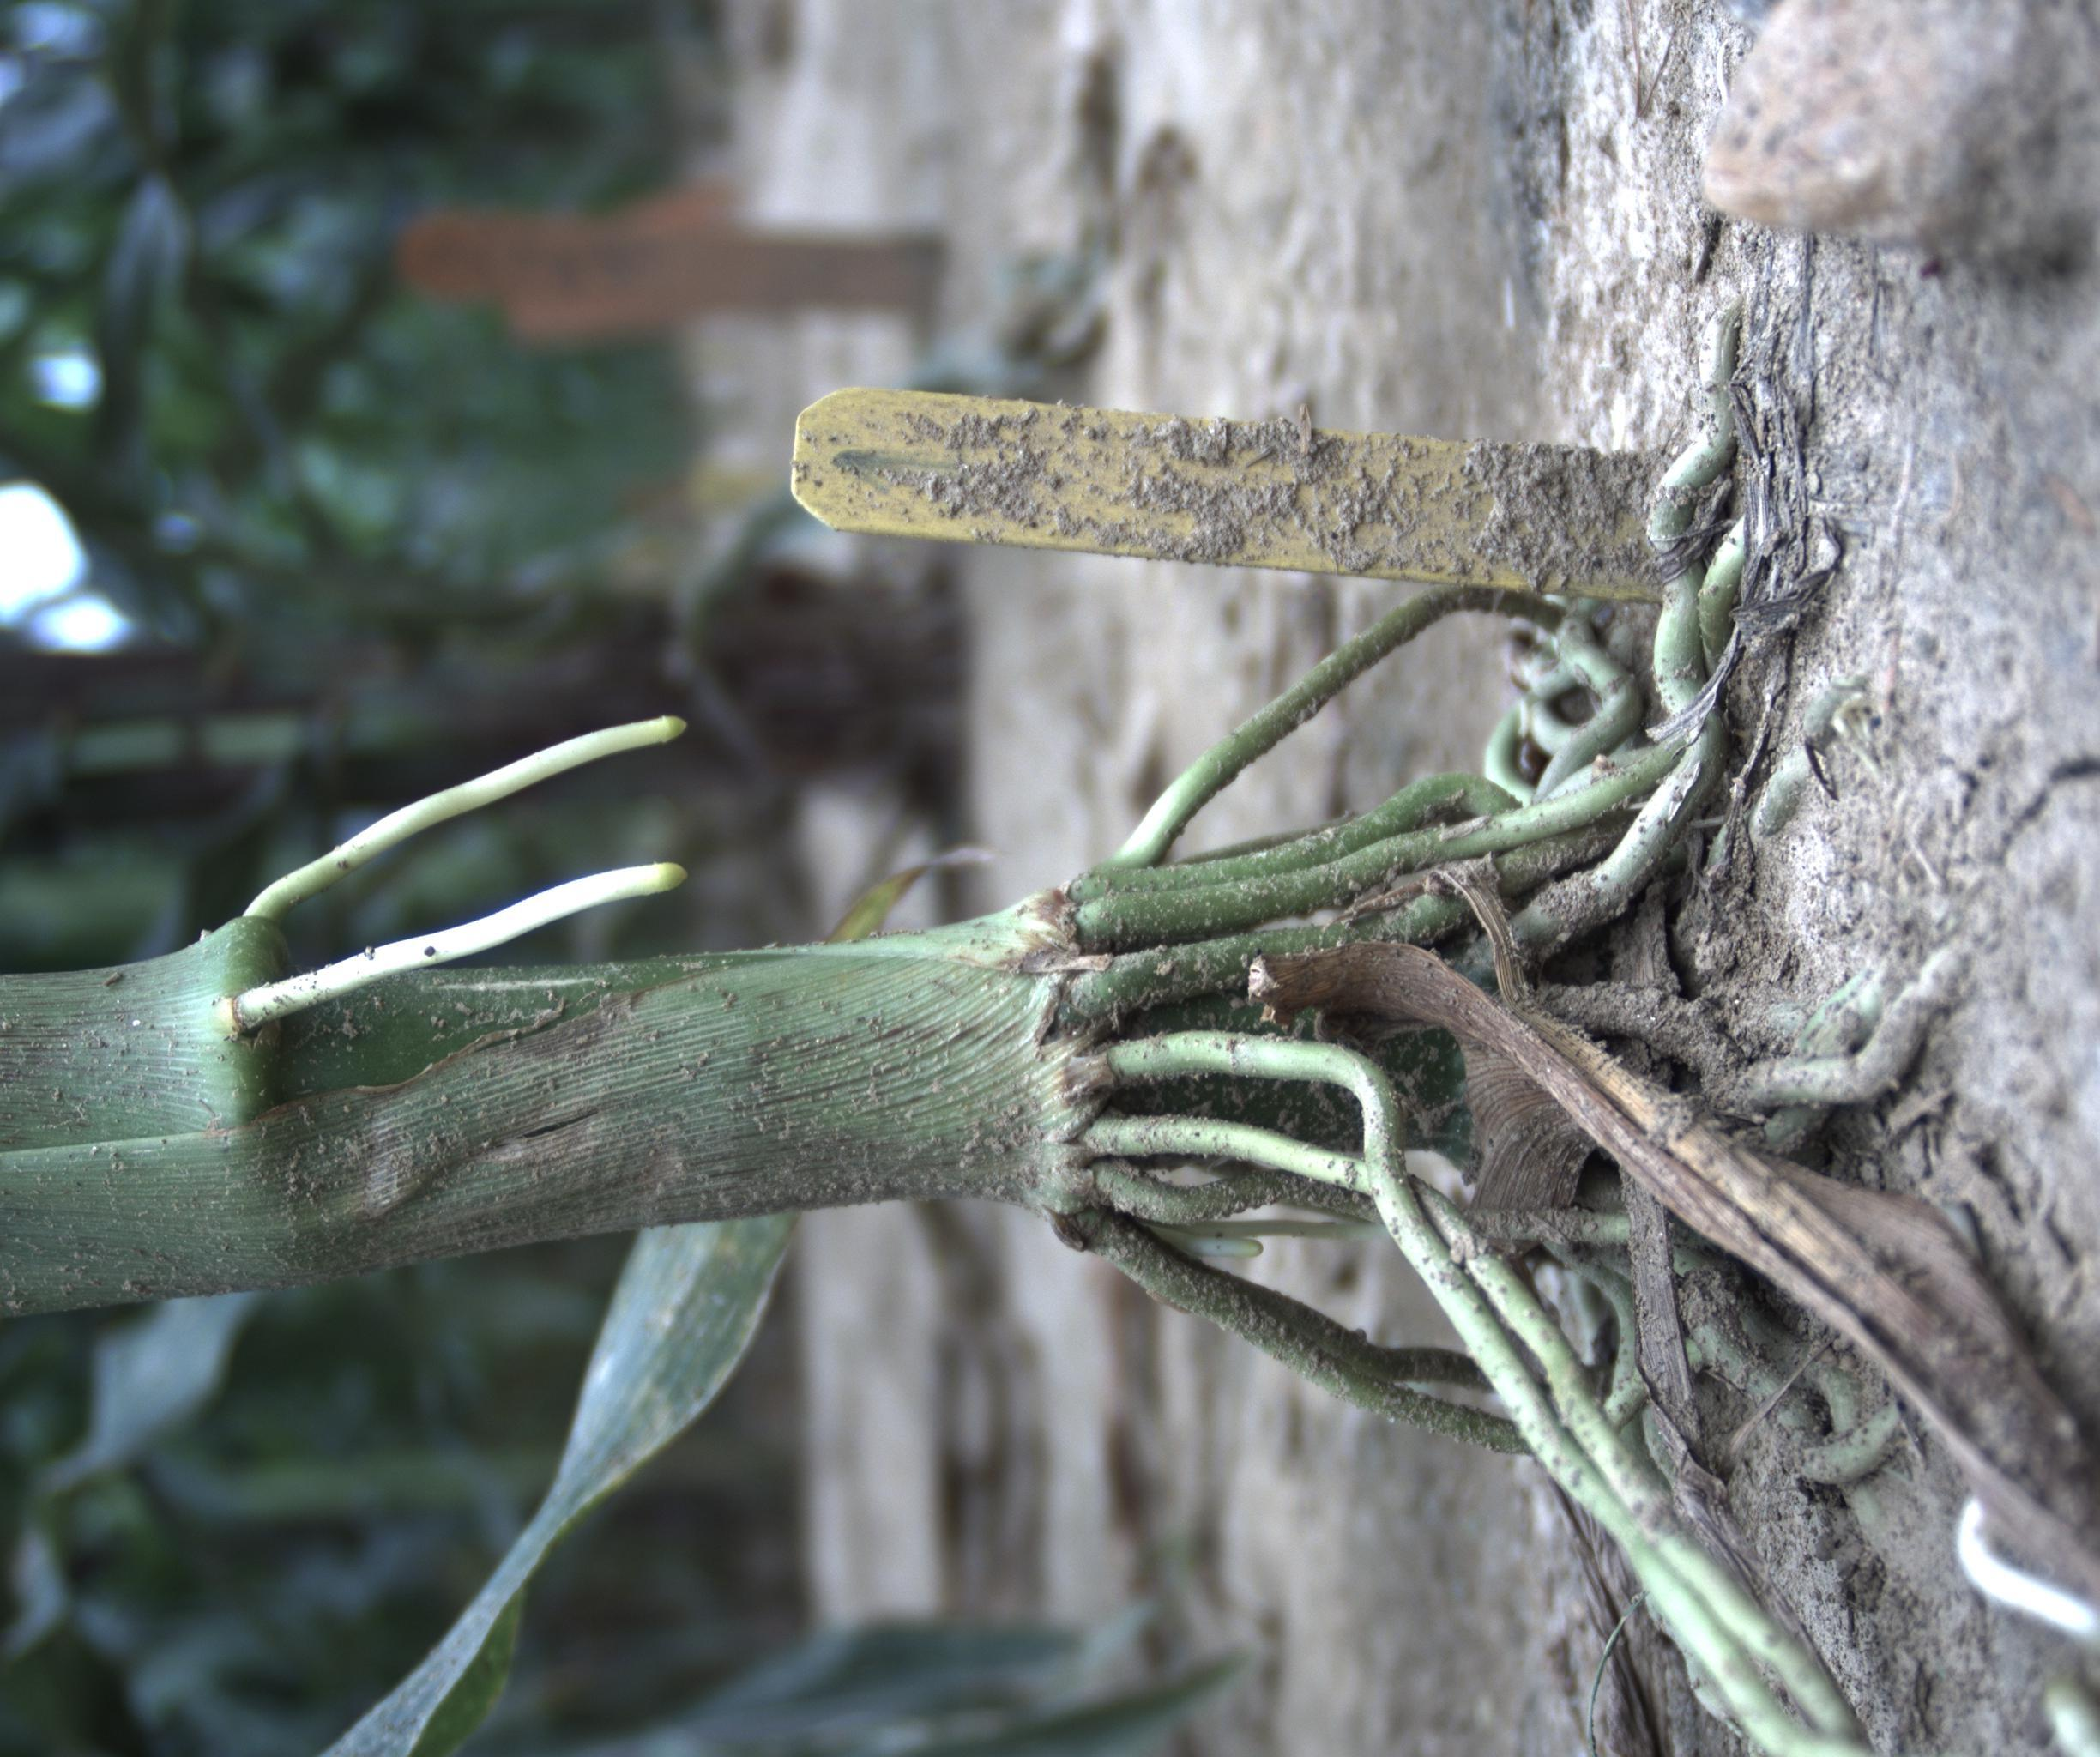
\includegraphics[width=\textwidth, angle=-90]{figures/w22.jpg}
    \end{minipage}
    \hfill
    \begin{minipage}{0.41\textwidth}
        \centering
        \includegraphics[width=\textwidth, angle=-90]{figures/TSH4.jpg}
    \end{minipage}
    \caption{TSH4 Mutants (right) show higher brace root counts than wild type (left) as well as more aerial brace roots and a secondary emergence pattern}
    \end{mdframed}
\end{figure}

With this in mind, it is hypothesized that TSH4 has a similar function in maize brace roots to its function in leaves and tassel bracts. That TSH4 acts as a stop signal and boundary for the organ development until the proper time for emergence. 

\section{Methods}
To test our hypothesis, we are seeking to follow some of the logic of Xiao et al.\cite{Xiao2022} We are using the CHipseq dataset from this paper and pairing it with out own whole node RNAseq analysis to see if the TSH4 targets are found in brace roots at each different stage of development. 

\subsection{CHiPseq}
The methods section of Xiao et al.\cite{Xiao2022} gives us this description of the CHiPseq experiment:
"Maize B73 plants were grown in the experimental field of the Plant Gene Expression Center, University of California Berkeley. Young ear primordia smaller than 5 mm were carefully dissected. About 1 g of tissue per biological replicate was fixed in 1 \% formaldehyde solution for 10 min under vacuum and quenched by adding glycine to a final concentration of 0.1 M. Nuclei extraction and ChIP using the TSH4 antibody were performed as described previously. \cite{Dong2019} Normal goat anti-rabbit IgG was used as a negative control. To validate the putative TSH4-binding targets, three biological replicates of immunoprecipitated DNA in ChIP were applied for each qPCR using respective primer pairs listed in table S13 (additional materials "xiao\_supplemental.xlsx") with Fast Evagreen qPCR mix. Relative enrichment was calculated using the $\delta$Ct (threshold cycle) method, and significant difference was evaluated through t test between anti-TSH4 ChIPed samples and IgG control." 
\subsection{Nodal RNAseq} 
For our nodal RNAseq dataset, samples from 3 nodes in each of 3 plant replicates were sequenced. Each of these 3 nodes representing a stage of brace root development. 


%begin Amaryllis-Methods
Samples were sent to Amaryllis Nucleics for processing and sequencing. RNA-seq libraries were prepared by using the Full Transcript mode YourSeq Dual (FT \& 3'-DGE) RNAseq Library Kit (Amaryllis Nucleics). A Bioanalyzer 2100 (Agilent, High Sensitivity DNA Kit) was used for library quality control, to determine average library size, and together with concentration data from a Qubit 2.0 Fluorometer (Life Technologies, dsDNA High Sensitivity Assay Kit) to determine individual library molarity and pooled library molarity. A PippinHT (Sage Science) was used for size selection to get pooled libraries 250-500 bp in length. These size-selected, pooled libraries were sequenced on a NextSeq 500 (Illumina, High Output v2 75 cycle kit) to yield single-read 80 bp reads. FASTQ sequence files were preprocessed in two steps. A Python library (clipper.py, https://github.com/mfcovington/clipper) was used to trim off the first 8 nucleotides of each read to remove potential mismatches to the reference sequence caused by annealing of a random hexamer required for library synthesis. Trimmomatic v0.36 \cite{Bolger2014} was used to remove adapter sequences and trim or filter reads based on quality. The parameters used for Trimmomatic were ILLUMINACLIP:TruSeq3-PE-2.fa:2:30:10 LEADING:3 TRAILING:3 SLIDINGWINDOW:4:15 MINLEN:50.

Preprocessed reads were mapped to the Zea mays B73 v4 genomic reference sequence \cite{nihMaysGenome} using HISAT2 \cite{HISAT2}. Read counts for each gene in the gene annotation file \cite{nihMaysGenome} were calculated using htseq-count (with the -s yes parameter to enforce strand-specific alignment) from the HTSeq Python library \cite{Anders2014}.

The R package edgeR \cite{edgeR} was used to identify genes differentially expressed between the three nodes of interest. Transcripts were retained for analysis if they had more than one count per million in at least three samples. After normalization factors were calculated and dispersion estimated, genewise negative binomial generalized linear models with quasi-likelihood tests were used to identify node effects across matched samples. Differentially expressed genes were then filtered using a false discovery rate (FDR) cutoff of 0.05. FDRs were calculated by adjusting P-values for multiple comparisons using the Benjamini–Hochberg procedure.
%end Amaryllis-Methods

The node highest on the plant, referred to as node 3, represents the Induction stage. This is the stage in which there are no observable brace root primordia. The second node from the ground, node 2, represents the initiation stage, where brace roots are just beginning to form emergence sights visible on the node. The lowest node to the ground, node 1, represents the Emergence stage, in which the brace roots have formed and are emerging from the plant and growing towards the soil.  
\begin{figure}[H]
    \centering
    \begin{mdframed}[backgroundcolor=green!20]
    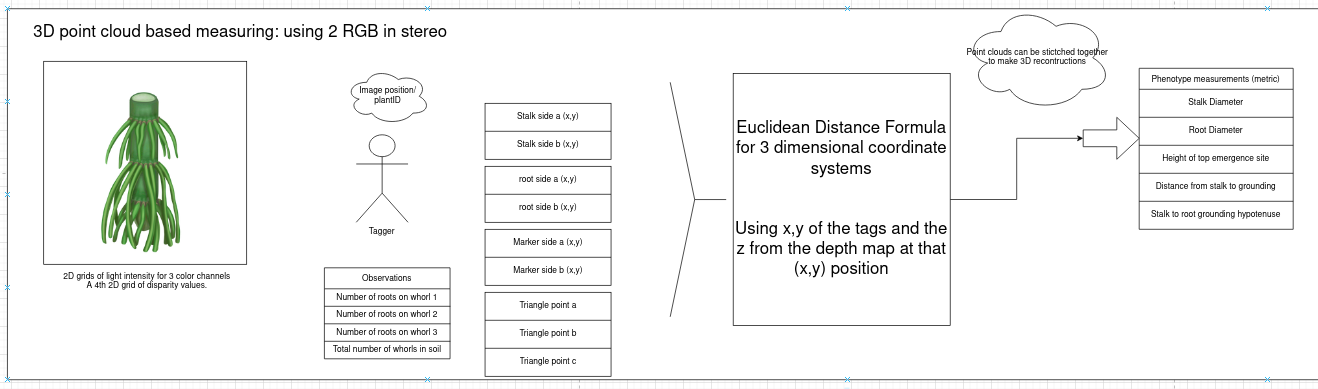
\includegraphics[width=1\linewidth]{figures/image.png}
    \caption{Stages of brace root development. Stage 1: Induction (signified as "node 3" in our analysis) shows no development. Stage 2: Initiation (signified as "node 2" in our analysis) shows when the brace root primordia start to form in the node. Stage 3: Emergence (signified as "node 1" in our analysis) shows when the brace root primordia emerges from the node. }
    \end{mdframed}
\end{figure}
\subsection{Enrichment analysis of differentially expressed TSH4 targets in brace root nodes}
The TSH4 Chipseq genes were converted from B73v3 to B73v4 using MaizeGDB gene mapping tool. \cite{Woodhouse2021} The converted list was used to filter each of the 3 DEG lists from RNAseq. Through a Venn diagram, the overlap gene set was divided into 7 subsets which were enriched through Agrigov2 \cite{Tian2017}. Gene ontology terms that were significantly enriched were noted and expression patterns for those genes were plotted in a heatmap of expression z-score.

\section{Results}
%Overlap Venn diagram
\subsection{TSH4 targets are differentially expressed between brace root nodes}
Of the 1392 TSH4 targets, 862 were present in our RNAseq dataset. 315 of those genes were differentially expressed between nodes with a log fold change of 1 or higher and an FDR below 0.05. \ref{fig:Venn1} shows a venn diagram of these gene sets. The overlap regions of this diagram signify subsets of interest because they are genes up or down regulated in a specific node. The regions on the perimeter of the diagram signify genes that transition between nodes or, in the case of the n3-n1 perimeter region, an end to end comparison. 
\begin{figure}[H]
    \centering
    \begin{mdframed}[backgroundcolor=green!20]
    \centering
    \includegraphics[width=.5\linewidth]{figures/venn_diagram.png}
    \caption{Venn diagram of TSH4 targets in nodal DEG list. Each of the 3 circles is a list of differentially expressed TSH4 targets. Naming for the sets includes the two nodes that were compared. Example: n3-n1 are DEG between node 3 (inductance) and node 1 (emergence)}
    \label{fig:Venn1}
    \end{mdframed}
\end{figure}

\subsection{Gene ontology reveals biological processes in brace root development}
%labeling the regions through GO report
For each of the 7 subsets of our overlapping gene set, only the epicenter of the venn diagram contained no significant GO annotations. The biological processes present in each subset confirms our logic previously described. The induction subset showed that there were large changes in anatomical structure morphogenisis (31 genes, GO:0009653) and post-embryonic development (28 genes, GO:0009791) to come in the next stages. The initiation subset showed no significant biological processes but showed changes in regulatory region nucleic acid binding (5 genes, GO:0001067) and transporter activity (10 genes, GO:0005212).  
The emergence subset contained clusters of GO terms indicating developmental growth involved in morphogenesis (9 genes, GO:0060560). Other ontology clusters include genes involved in the reproductive process (21 genes, GO:0022414), regulation of hormone levels (9 genes, GO:0010817) and steroid biosynthesis (5 genes, GO:0006694). The perimeter regions align well with transitions between stages of brace root development with changes from induction to initiation showing the beginnings of lateral organ development and changes from initiation to emergence being marked with regulation of gene expression. The end to end comparison marked significant changes in metabolism and cell signaling.   
\subsection{Expression patterns of TSH4 \& signalling pathways suggest regulation}
Expression of TSH4 is very high in inductance becomes down regulated in initiation and is not significantly expressed in emergence. This mirrors the pattern found in tassel bracts and suggests that TSH4 is suppressing brace root development. In tassel bracts, two signalling pathways, gibberellin and auxin, are found to be attenuated by TSH4 while abscisic acid is promoted.\cite{Xiao2022} In brace roots we do not see the same hormone signals but we do see signals involved in root growth: Ethylene, auxin, and brassinosteroids. In \ref{fig:meta-express} we can see that ethylene and brassinosteroids have an inverse expression pattern to TSH4, this suggests a suppression interaction.  
\begin{figure}[H]
    \centering
    \begin{mdframed}[backgroundcolor=green!20]
    \centering
    \includegraphics[width=.95\linewidth]{figures/Hormonal_expression_heatmap.png}
    \caption{Expression heatmap (by z-score) across nodes shows that TSH4 expression is high in node 3 and metabolic signals such as BRS1 (Brassinosteriod synthesis 1) and EREB118 (ethylene responsive element binding protein 118) show an inverse expression pattern to TSH4. In contrast to tassle bracts, Auxin response factor transcription factors (ARFTF) are co-expressed with TSH4}
    \label{fig:meta-express}
    \end{mdframed}
\end{figure}
\subsection{The presence of other transcription factors suggest a regulatory network}
In \ref{fig:meta-express} we saw a auxin response factor transcription factors were highly expressed with TSH4 in the induction stage of brace root development. But there are also other transcription factors that have interesting expression patterns. Notably, myoblastosis transcription factor 99 (MYB99) and heatshock transcription factor 18 (HSFTF18) have the inverse expression pattern of TSH4. MYB99 is a key transcription factor in regulating secondary metabolic processes. \cite{Cao2020} HSFTF18 has also been found to be expressed in brace roots. \cite{Li2019} 
\begin{figure}[H]
    \centering
    \begin{mdframed}[backgroundcolor=green!20]
    \centering
    \includegraphics[width=.95\linewidth]{figures/TF_expression_heatmap.png}
    \caption{Expression heatmap (by z-score) across nodes shows that TSH4 expression is high in node 3 and the presence of other TFs show that there may be more complicated regulation networks at play.}
    \label{fig:meta-express}
    \end{mdframed}
\end{figure}


\section{Discussion}
More work is required in order to find the exact mechanisms of tassel sheath 4's regulation of brace root development. But this data does suggest that a similar pattern to the one in tassel bracts. We see suppression of many genes involved in organ development and massive metabolic and signalling changes throughout all three stages. It should be noted that a good way to improve this study is to get both sequencing data sets from the same part of the plant, ie. running the CHiPseq experiment using brace root tissue. This could filter out TSH4 targets that are specific to flowering. Another possible way to continue from this point would be to try to find possible links in the regulatory chain by trying to predict interactions amongst the un-characterized gene products in this data set. With this in mind, the results of this project show promising evidence for a regulatory network around brace root development and justifies further investigation.   




\printbibliography

